\documentclass{cmspaper}
\usepackage{graphicx}
\begin{document}

\begin{titlepage}

     \internalnote{2008-xxx}
     \date{8 March 2009}
     \title{Pixel Online Software and Pixel Detector Control Software Integration}
     \begin{Authlist}
      Souvik Das
       \Instfoot{cornell}{Cornell University, Ithaca, NY}
     \end{Authlist}
 \submitted{}
 \collaboration{}
 \conference{}
 
 \begin{abstract}

The Online Software for the CMS Pixel Detector is designed to work in close coordination with the Detector Control System framework to provide an automatic detector power-up procedure and swift reaction in the online software to current, temperature and other detector condition trips.

 \end{abstract}
 
 \note{} 
 
\end{titlepage}


\section{Introduction}

The CMS Pixel Online Software is primarily responsible for programming, calibrating and monitoring the front-end and readout electronics of the CMS Pixel Detector. It may be operated through its own web-interface on any generic web browser, or through the central Run Control of the CMS Experiment. It is based on a cross platform data acquisition framework called XDAQ. A detailed description of the CMS Pixel Online Software is available in Internal Notes.

The CMS Pixel Detector Control System software is responsible for setting and monitoring the voltages, currents, temperatures, humidities and other conditions data of the CMS Pixel Detector.

While the Pixel Online Software and the Detector Control Software discharge their more or less independent responsibilities, two outstanding challenges demand some measure of integration between them:

\begin{enumerate}
\item Automation of the power-up sequence.
\item Monitoring of detector conditions data for swift reaction to changes and notification to central Run Control
\end{enumerate}

Automation of the power-up sequence must account for the peculiarities of the Forward Pixel (FPix) and the Barrel Pixel (BPix) detectors while configuring the front-end and readout electronics. They are described in Section ~\ref{sect:peculiarities}.

Monitoring must do interesting things too XXX.

All of this must be done within the existing and accepted framework of the Pixel Online Software and the Detector Control System software. A brief detour through the salient features of these two software worlds are necessary to appreciate their integration and are described in Sections ~\ref{sect:pos} and ~\ref{sect:dcs} respectively.


\section{Pixel Online Software} \label{sect:pos}

The Pixel Online Software is organized as a hierarchy of XDAQ applications. The top level XDAQ application, \textit{PixelSupervisor}, is interfaced to the central Run Control through the RCMS application, \textit{PixelFunctionManager}. This is depicted in Figure {1}.

\textit{PixelSupervisor}, \textit{PixelTKFECSupervisor}, \textit{PixelFECSupervisor} and \textit{PixelFEDSupervisor} are formally required to work within the constraints of a Finite State Machine whose states must be a superset of the set of states in the Finite State Machine prescribed in the Level 1 Function Manager document.

\subsection{PixelSupervisor}

\textit{PixelSupervisor} is the XDAQ application that coordinates the underlying Supervisors to configure, calibrate and acquire data from the detector. It has the Finite State Machine depicted in Figure {X}.

\subsection{PixelTKFECSupervisor}

\textit{PixelTKFECSupervisor} is a XDAQ application used to program the slow-$I^{2}C$ devices like the portcard XXX and CCU XXX via the Tracker Front End Controller (tkFEC) VME board. It may also be used to monitor the DCU temperatures. One instance of the \textit{PixelTKFECSupervisor} is designed to control one tkFEC board. There are two tkFEC boards for the CMS Pixel Detector, one for the FPix and one for the BPix, and hence two instances of \textit{PixelTKFECSupervisor} are required for all slow-$I^{2}C$ programming.

The portcards and CCUs that will be programmed must have their voltages turned on before the tkFEC may be used to program them.

The \textit{PixelTKFECSupervisor} has the Finite State Machine depicted in Figure {X}.

\subsection{PixelFECSupervisor}

\textit{PixelFECSupervisor} is a XDAQ application used to program the Token Bit Manager chips (TBM) and Readout Chips (ROC) through Pixel Front End Controller (pFEC) VME boards. One instance of \textit{PixelFECSupervisor} is designed to manage one crate of pFEC boards. There are three pFEC boards for the CMS Pixel Detector, one for the FPix and two for the BPix. The two pFECs for the BPix inhabit the same the crate while the pFEC for the FPix lives in another. Therefore, two \textit{PixelFECSupervisors} are sufficient for the detector.

It has the Finite State Machine depicted in Figure {X}.

\subsection{PixelDCSFSMInterface}

\textit{PixelDCSFSMInterface} is a XDAQ application that relays the FSM state of the PVSS(?) system for various power coordinates to the \textit{PixelFECSupervisors} and \textit{PixelTKFECSupervisor}.


\section{Pixel Detector Control System Software} \label{sect:dcs}

\section{Peculiarities of Forward and Barrel Pixel Power Up} \label{sect:peculiarities}

Historically...

\subsection{Portcards and CCUs}

Portcards and CCUs can either be powered on or off. It does not matter whether they belong to the FPix or the BPix. Hence the \textit{PixelTKFECSupervisors}, which program them, need to be aware of their binary state before programming them. They need to be programmed to ensure the correct timing of the fast-$I^{2}C$ commands for programming the ROCs and TBMs.

\begin{table}[htb]
	\centering
		\begin{tabular}{|c|c|c|c|c|}
			\hline
			                  & \textbf{OFF Voltage} & \textbf{ON Voltage} & \textbf{Ramp Up} & \textbf{Ramp Down} \\
 \hline
		  \textbf{Portcard} &    0 V      &     2.6 V     &         &            \\
\hline
		  \textbf{CCU}      &    0 V      &     2.6 V     &         &            \\
		  \hline
		\end{tabular}
\end{table}

\subsection{Readout Chips}

Readout Chips have three primary voltages that need to be turned on or off: the analog voltage (\emph{Vana}), the digital voltage (\emph{Vdigi}) and the bias high voltage (\emph{HV}). The analog current (\emph{Iana}) may also be monitored as it changes when the DACs on the ROC are loaded.

The \emph{Vdigi} of all BPix ROCs can either be \textbf{LV\_OFF} at 0 V or \textbf{LV\_ON} at 2.6 V. However, the \emph{Vdigi} of all FPix ROCs can either be \textbf{LV\_OFF} at 0 V, \textbf{LV\_ON\_REDUCED} at 2.1 V or \textbf{LV\_ON} at 2.6 V. The DACs of the FPix ROCs must be programmed at \textbf{LV\_ON\_REDUCED} once to make sure the currents are within acceptable limits before ramping them up to \textbf{LV\_ON} and programming their Mask and Trim bits.

\emph{Vana} of all ROCs can either be \textbf{OFF} at 0 V, or \textbf{ON} at 1.6 V. Its voltage is ramped up at ... V/sec and ramped down at ... V/sec.

\emph{HV} for all ROCs can either be \textbf{OFF} at 0 V or \textbf{ON} at ~ 200 V.

\section{The Detector Power Up Sequence}

For the power-up sequence, the detector is broken down into 8 power coordinates as shown in Fig.~\ref{fig:powerPartition}.

\begin{figure}[h]
\centering
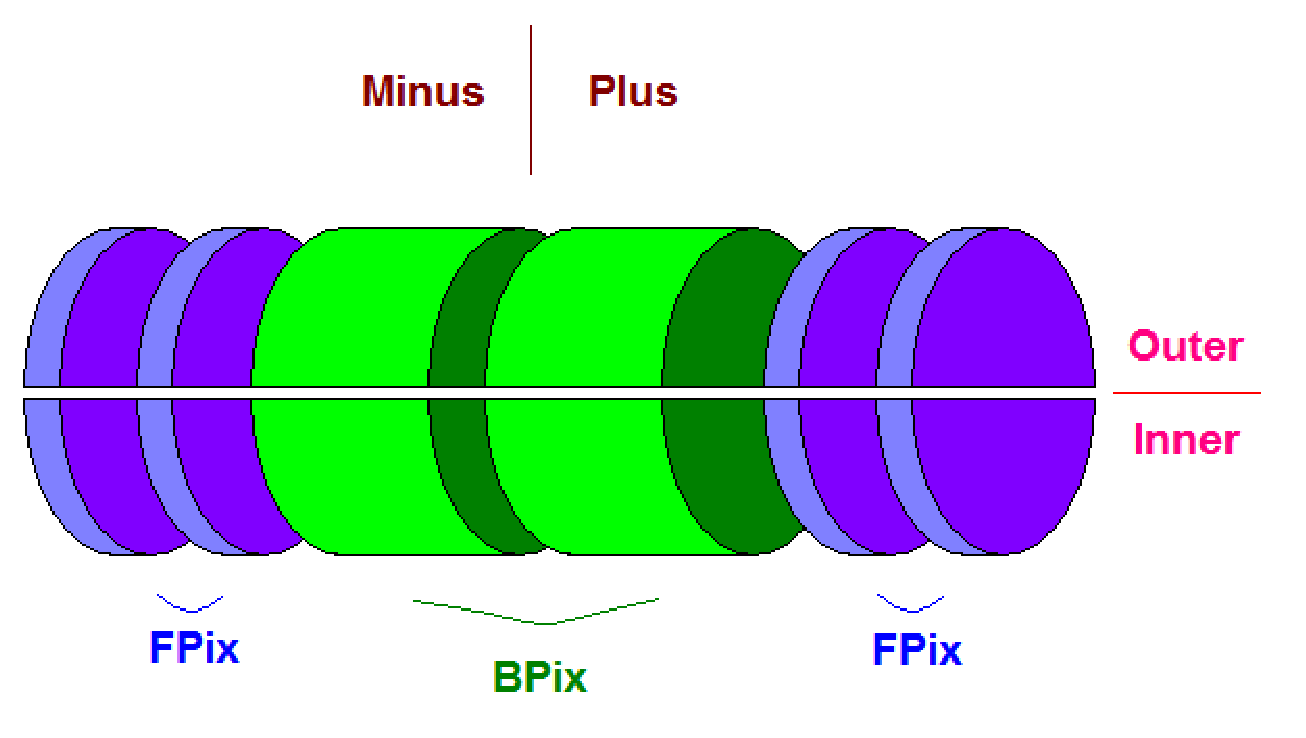
\includegraphics[width=0.75\linewidth]{powerPartition.eps}
\caption{Division of the detector into 8 power coordinates.}
\label{fig:powerPartition}
\end{figure}




\section{Monitoring Conditions Data}



\end{document}
